
\begin{center}
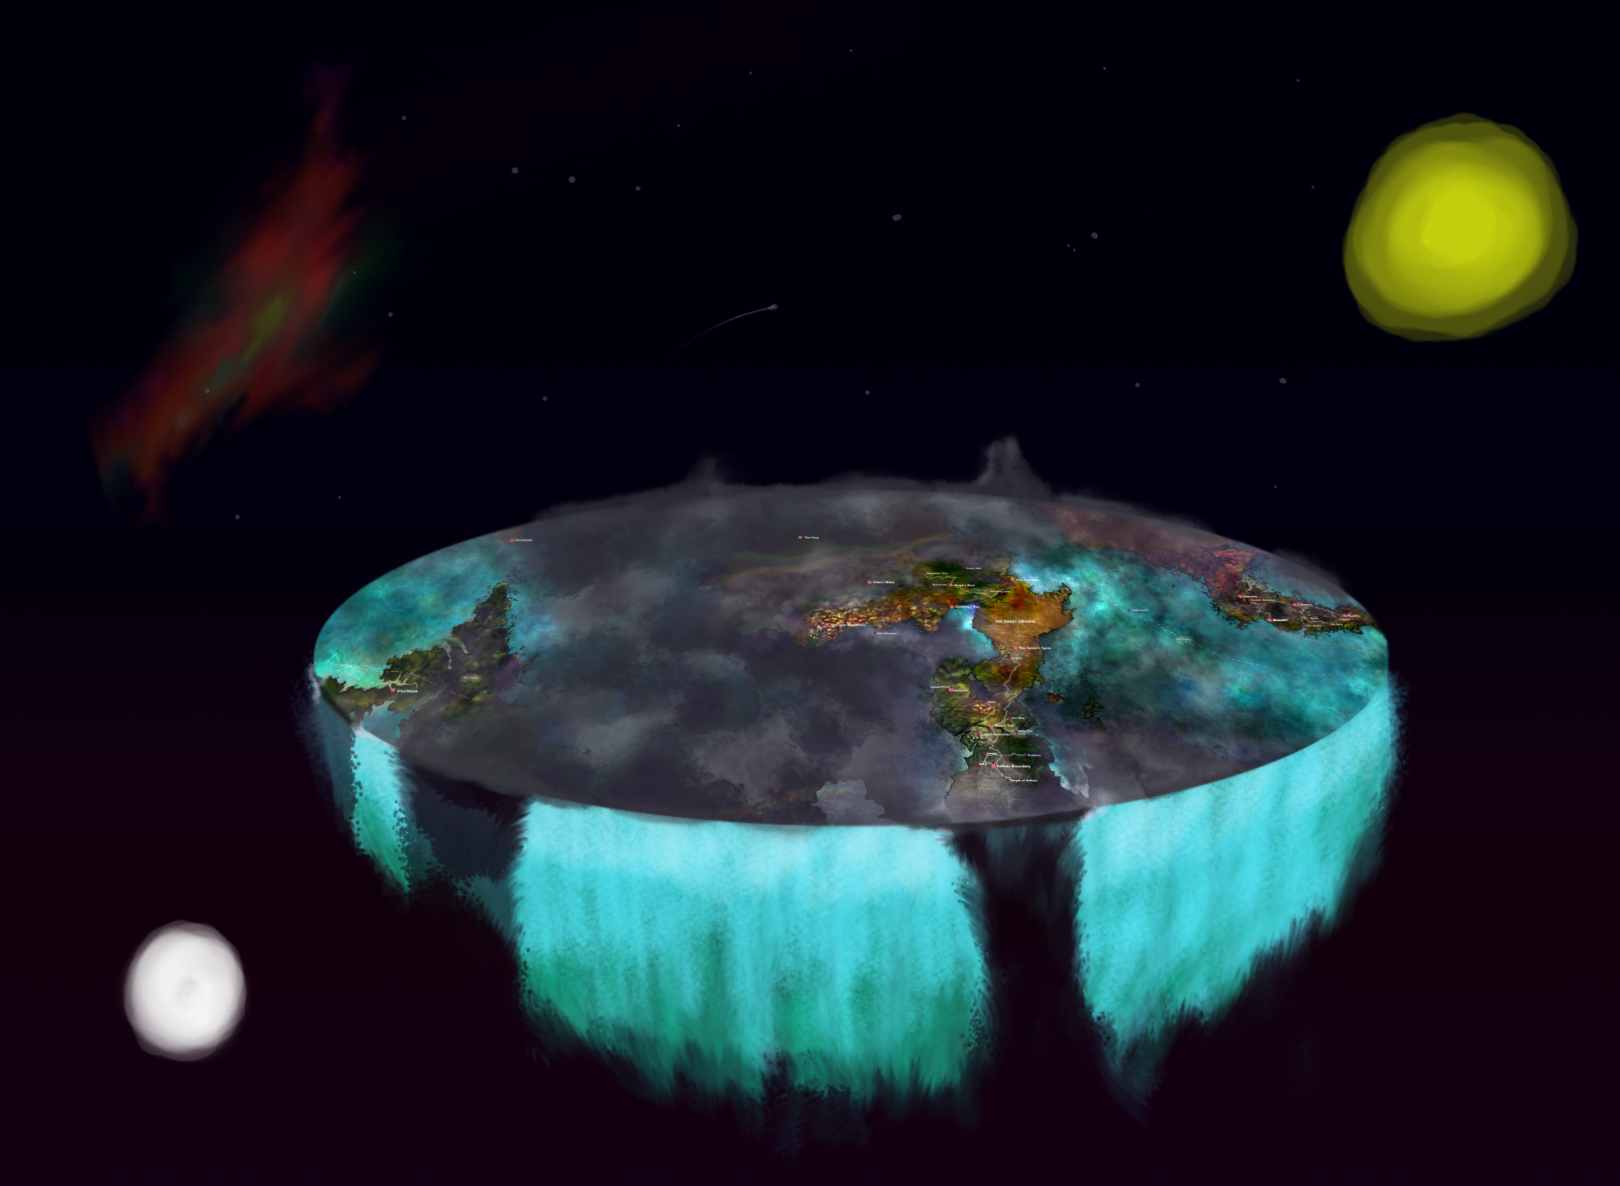
\includegraphics[width=\textwidth]{./content/img/flatVelterra.png}
\begin{figure}[h]
\end{figure}
\end{center}

\begin{multicols}{2}

\section{Background}

\subsection*{The Story So Far}

In the world of Velterra, domain of the Seven, the Church rules all through faith, fear, and the filtered power of absent gods.  But the gods are not merely distant --- they have been sealed away, their power sundered from the world by the Church's own hand centuries ago.  What was meant as protection has become a prison, and the Church that once served the light has become corrupt, sending countless innocent souls to Hell through its ever-expanding definition of sin.

In Hell, a bureaucratic devil named Lazarus hatches a desperate plan.  Overwhelmed by the flood of undeserving damned, he reaches into the mortal world and plucks five recently deceased souls from the edge of oblivion --- a gun-toting dwarf pastor, a pair of goblin twins, a disgraced Book Burner, and a mysterious foreign swordswoman.  He offers them a deal: a second chance at life, in exchange for a mission to destroy the Church and break the seal that imprisons the gods.

The group's journey takes them from the frozen wastes of the south to the great city of Hope's Rest, across burning deserts and treacherous seas, through ancient towers and foreign wars.  Along the way they gain and lose companions, build a guild, found a bank, acquire an airship, and slowly uncover the truth about their world --- that the gods are not dead, merely locked out, and that the key to saving everything lies in reuniting the world with its creators.

This is their story.  These are the episodes as they were lived, told in the words of those who were there.

\begin{DndReadAloud}
``You have all recently died.  You have been brought together, here, and given a second chance at life in exchange for carrying out a mission to destroy the Church.''

--- Lazarus, to the newly resurrected party
\end{DndReadAloud}

\end{multicols}

\clearpage
